\chapter{Analyse, Fortolkning og resultateri}
\label{Ch:4}

I dette afsnit skal vi se på det data materiale som er blevet indsamlet i forbindelse med hhv. spørgeskemaet og de skriftlige produkter. 

\section{Spørgeskemaet}
\label{Sec:4.1}

I dette afsnit belyses den empiri som er blevet indsamlet med Survey-Xact forud for elevernes skriveproces. Spørgeskemaet har indsamlet 117 besvarelser og er gennemført udelukkende i 1.g STX klasser på Viborg Katedralskole, hvilket betyder at der har været mulighed for at indhente 349 besvarelser, dermed har undersøgelsen haft en svar procent på 33,5 \%. Der kan derfor med rimelighed tillægges værdi til de svar som eleverne giver på spørgsmålene da vi har svar fra lidt mere end en tredje del af eleverne på skolens 1.g-årgang. Eleverne har skullet vurderer 5 udsagn på en skala fra 1 til 7. På denne skala var 1 meget uenig med udsagnet mens 7 var meget enig i udsagnet. Betagter man den indkomne emperi fra spørgskemaet, se figur \vref{fig:4.1.a}. Af figuren fremgår det, at eleverne vurderer det praktiske arbejde som motiverende. 
\begin{figure}[h!]
	\centering
	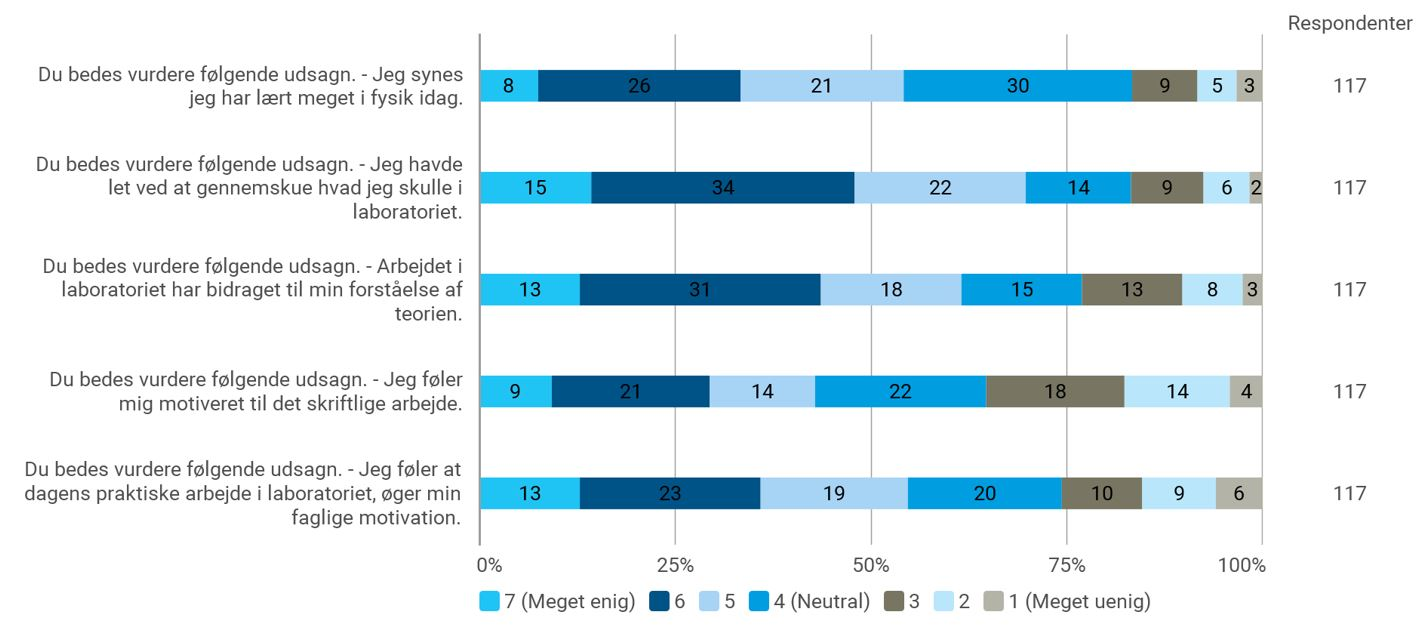
\includegraphics[width=0.9\textwidth]{Figs/Sammenlign}
	\caption{Det samlede datasæt for de fem spørgsmål med hver 117 respondenter fra en 1.g årgang på Viborg Katedralskole. Svar procenten for undersøgelsen er på omkring 33 \%. }
	\label{fig:4.1.a}
\end{figure}
Kigger man på antallet af positive svar på de fem udsagn hvor eleverne har valgt 4 eller højere så er gennemsnittet af de fem målinger 66,32 \%. Man kan så diskuterer om eleverne har forstået spørgsmålene som de var tænkt. Hvad menes der fx med spørgsmålet ``Jeg synes jeg har lært meget i fysik idag.'' - Her lægges der op til en subjektiv vurdering af hvad der menes med at lære meget. Dette kan medfører at der er en hvis spredning i svarende fordi eleverne ikke nødvendigvis måler sig op imod den samme målestok. Men som det fremgår af figur \vref{fig:4.1.b} har 83 \% vurderet neutral eller bedre på dette udsagn - hvilket må tolkes som om eleverne faktisk har lært noget. 

Her kunne det være interessant at undersøge om der vil være et lignende billede hvis man spurgte eleverne om det samme i en almindelig teori-time hvor eleverne ikke nødvendigvis arbejder paktisk med den undersøgende tilgang. Gjorde man dette ville man kunne få et hint om hvorvidt det er det praktiske arbejde eller om eleverne generelt mener de lærer noget af fysik faget.
\begin{figure}[h!]
	\centering
	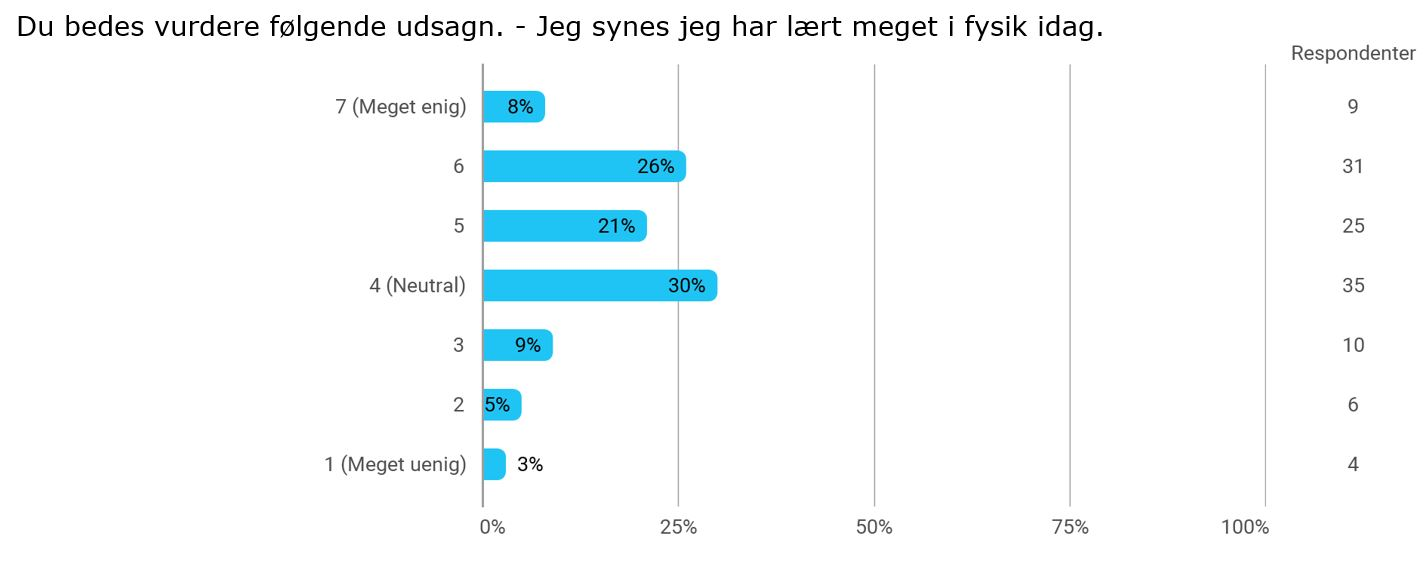
\includegraphics[width=0.9\textwidth]{Figs/Sp1}
	\caption{Spørgeskema svar til vurderingen af udsagnet ``Jeg synes jeg har lært meget i fysik idag.'' Her ses en klar positiv vægtning hvor 83 \% af respondenterne har svaret neutral eller bedre.}
	\label{fig:4.1.b}
\end{figure}



%\begin{figure}[h!]
%	\centering
%	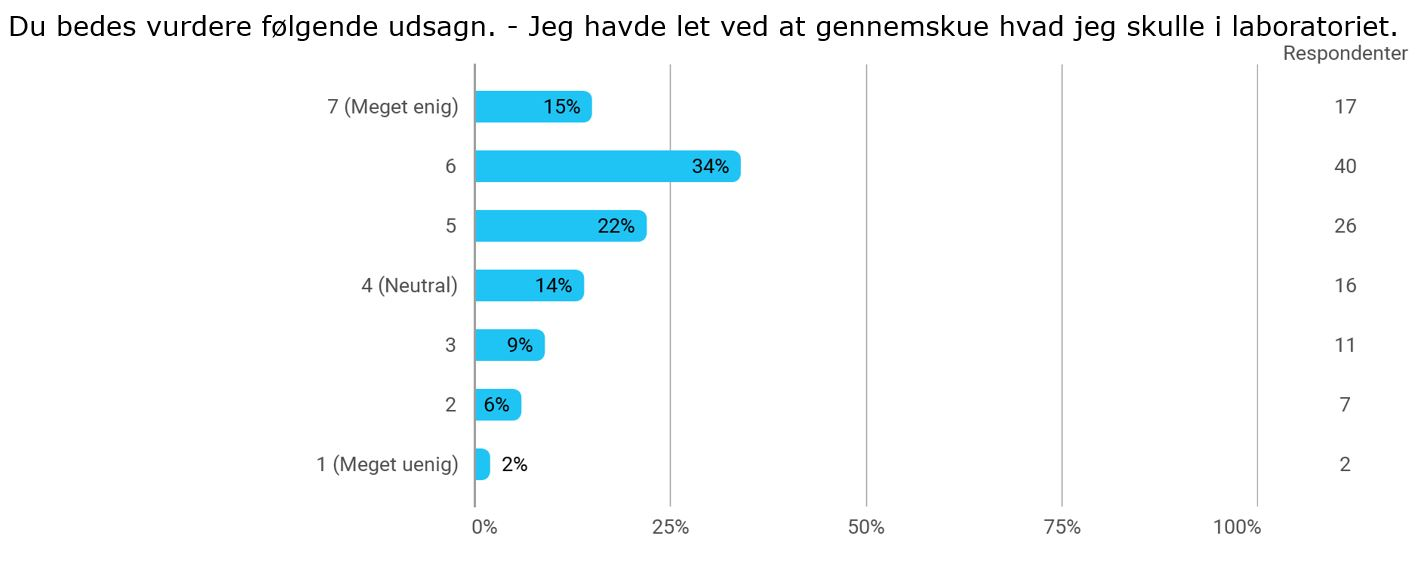
\includegraphics[width=0.9\textwidth]{Figs/Sp2}
%	\caption{Spørgeskema svar fra spørgsmål 2}
%	\label{fig:4.1.c}
%\end{figure}
%
%\begin{figure}[h!]
%	\centering
%	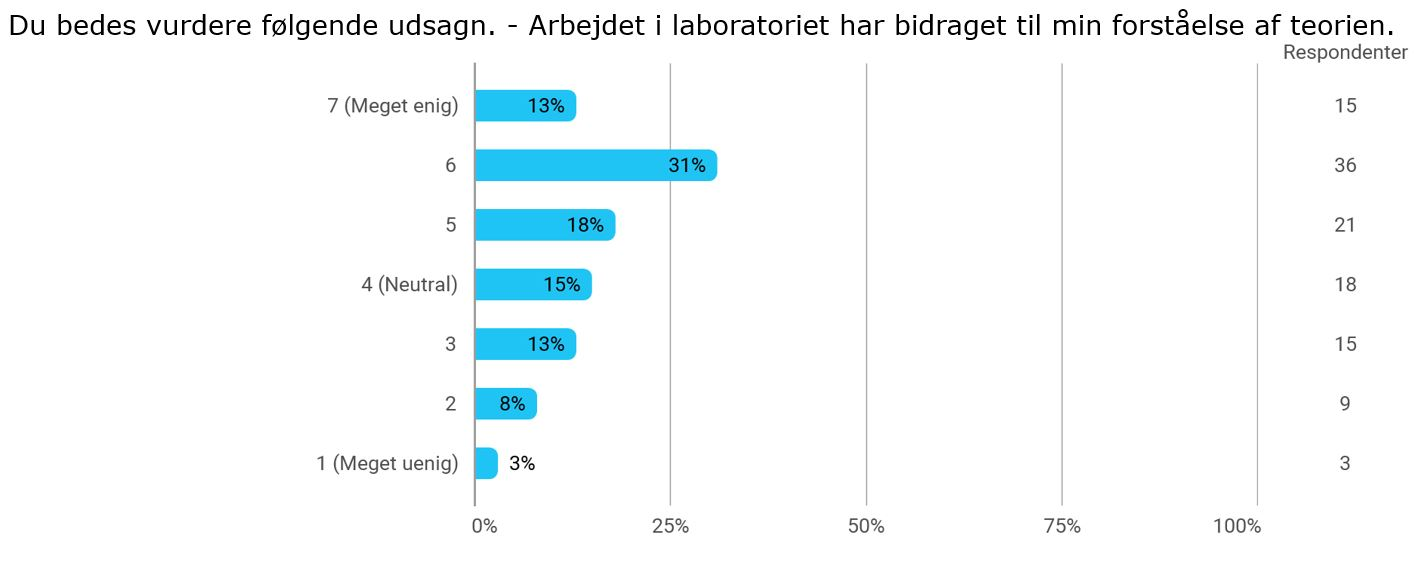
\includegraphics[width=0.9\textwidth]{Figs/Sp3}
%	\caption{Spørgeskema svar fra spørgsmål 3}
%	\label{fig:4.1.d}
%\end{figure}
%
%\begin{figure}[h!]
%	\centering
%	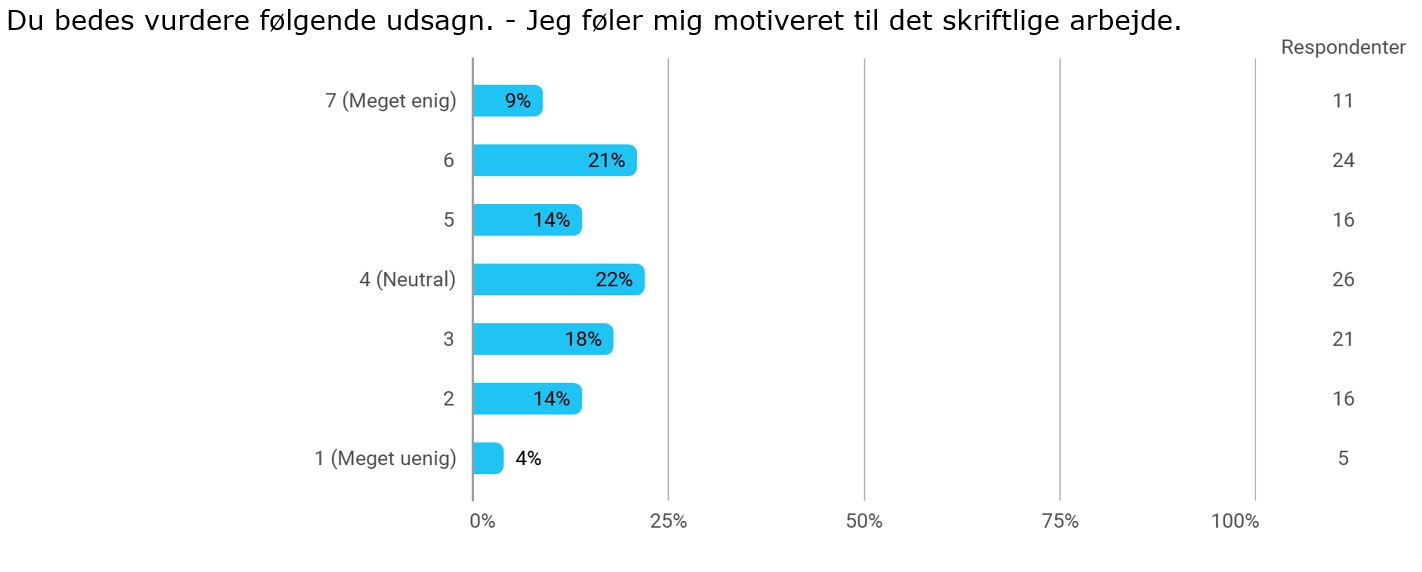
\includegraphics[width=0.9\textwidth]{Figs/Sp4}
%	\caption{Spørgeskema svar fra spørgsmål 4}
%	\label{fig:4.1.e}
%\end{figure}
%
%\begin{figure}[h!]
%	\centering
%	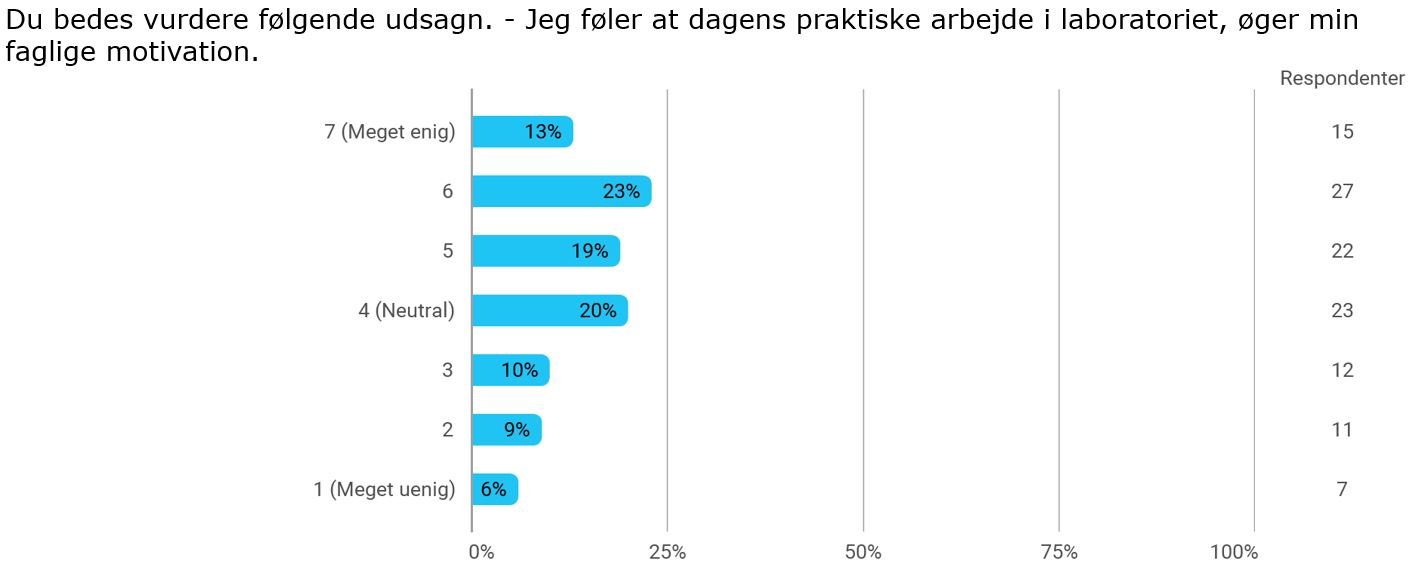
\includegraphics[width=0.9\textwidth]{Figs/Sp5}
%	\caption{Spørgeskema svar fra spørgsmål 5}
%	\label{fig:4.1.f}
%\end{figure}
